\documentclass[a4paper, twocolumn]{article}
\usepackage{booktabs}

%%%%%%%%%%%%%%%%%%%%%%%%%%%%%%%%%%%%%%%%%%%%%%%%%%%%%%%%%%%%%%%%%%%%%%%%%%%%%%
%%%%%%%%%  DO NOT EDIT !
%%%%%%%%%  DO NOT EDIT !
%%%%%%%%%  DO NOT EDIT !
%%%%%%%%%  DO NOT EDIT !
%%%%%%%%%  DO NOT EDIT !
%%%%%%%%%  DO NOT EDIT !
%%%%%%%%%%%%%%%%%%%%%%%%%%%%%%%%%%%%%%%%%%%%%%%%%%%%%%%%%%%%%%%%%%%%%%%%%%%%%%

\usepackage[english]{babel}
\usepackage{graphicx}             
\usepackage{tabularx}             
\usepackage{multirow}             
\usepackage{url}                 
\usepackage[ansinew]{inputenc}
\usepackage[small,bf]{caption}   
\usepackage{parskip}
\usepackage{amsmath}             
\usepackage{xcolor}
\usepackage{lipsum} 
 
%%%%%%%%%%%%%%%%%%%%%%%%%%%%%%%%%%%%%%%%%%%%%%%%%%%%%%%%%%%%%%%%%%%%%%%%%%%%%%
% fonts
%%%%%%%%%%%%%%%%%%%%%%%%%%%%%%%%%%%%%%%%%%%%%%%%%%%%%%%%%%%%%%%%%%%%%%%%%%%%%%

\usepackage{mathptmx}


%%%%%%%%%%%%%%%%%%%%%%%%%%%%%%%%%%%%%%%%%%%%%%%%%%%%%%%%%%%%%%%%%%%%%%%%%%%%%%
% spacing and indents
%%%%%%%%%%%%%%%%%%%%%%%%%%%%%%%%%%%%%%%%%%%%%%%%%%%%%%%%%%%%%%%%%%%%%%%%%%%%%%

\setlength{\parskip}{2pt}

%%%%%%%%%%%%%%%%%%%%%%%%%%%%%%%%%%%%%%%%%%%%%%%%%%%%%%%%%%%%%%%%%%%%%%%%%%%%%%
% geometry
%%%%%%%%%%%%%%%%%%%%%%%%%%%%%%%%%%%%%%%%%%%%%%%%%%%%%%%%%%%%%%%%%%%%%%%%%%%%%%

\usepackage[left=1.7cm,right=1.7cm,top=2.5cm,bottom=2.5cm]{geometry}
\setlength{\columnsep}{0.6cm}

%%%%%%%%%%%%%%%%%%%%%%%%%%%%%%%%%%%%%%%%%%%%%%%%%%%%%%%%%%%%%%%%%%%%%%%%%%%%%%
% make a header
%%%%%%%%%%%%%%%%%%%%%%%%%%%%%%%%%%%%%%%%%%%%%%%%%%%%%%%%%%%%%%%%%%%%%%%%%%%%%%

\usepackage{fancyhdr}
 
\pagestyle{fancy} 
\fancyhf{}  
\fancyhead[L]{\small\itshape Proceedings of the $9^{th}$ Conference on Interdisciplinary Musicology -- CIM14.
Berlin, Germany 2014}  
\fancyhead[C]{}  
\fancyhead[R]{}  
\renewcommand{\headrulewidth}{0.0pt}  
\fancyfoot[C]{}  
\renewcommand{\footrulewidth}{0.0pt}  

\pagestyle{fancy}

\makeatletter
\let\ps@plain\ps@fancy 
\makeatother
 
%%%%%%%%%%%%%%%%%%%%%%%%%%%%%%%%%%%%%%%%%%%%%%%%%%%%%%%%%%%%%%%%%%%%%%%%%%%%%%
% adjust titles
%%%%%%%%%%%%%%%%%%%%%%%%%%%%%%%%%%%%%%%%%%%%%%%%%%%%%%%%%%%%%%%%%%%%%%%%%%%%%%

\usepackage{titlesec}
  
\titleformat{\section}{\centering\normalfont\bfseries\sc\fontsize{10}{10}\selectfont}{\thesection.}{0.5em}{}
\titleformat{\subsection}{\normalfont\itshape\fontsize{10}{10}\selectfont}{\thesubsection.}{0.5em}{}
  
\titlespacing{\section}{0pt}{9pt}{2pt}
\titlespacing{\subsection}{0pt}{5pt}{0pt}
 
%%%%%%%%%%%%%%%%%%%%%%%%%%%%%%%%%%%%%%%%%%%%%%%%%%%%%%%%%%%%%%%%%%%%%%%%%%%%%%
% Strongly discourage hyphenation
%%%%%%%%%%%%%%%%%%%%%%%%%%%%%%%%%%%%%%%%%%%%%%%%%%%%%%%%%%%%%%%%%%%%%%%%%%%%%%

\hyphenpenalty=5000
\tolerance=1000

%%%%%%%%%%%%%%%%%%%%%%%%%%%%%%%%%%%%%%%%%%%%%%%%%%%%%%%%%%%%%%%%%%%%%%%%%%%%%%
% hyperref
%%%%%%%%%%%%%%%%%%%%%%%%%%%%%%%%%%%%%%%%%%%%%%%%%%%%%%%%%%%%%%%%%%%%%%%%%%%%%%

\usepackage{hyperref}

\hypersetup{
     unicode=false,           
    pdftoolbar=true,        
    pdfmenubar=true,        
    pdffitwindow=false,      
    pdfstartview={FitH},     
    pdftitle={},     
    pdfauthor={},      
    pdfsubject={},   
    pdfcreator={},   
    pdfproducer={},  
    pdfkeywords={keyword1} {key2} {key3}, 
    pdfnewwindow=true,      
    colorlinks=true,        
    linkcolor=darkgray,          
    citecolor=darkgray,         
    filecolor=darkgray,      
    urlcolor=darkgray            
}

%%%%%%%%%%%%%%%%%%%%%%%%%%%%%%%%%%%%%%%%%%%%%%%%%%%%%%%%%%%%%%%%%%%%%%%%%%%%%%
% abstract settings
%%%%%%%%%%%%%%%%%%%%%%%%%%%%%%%%%%%%%%%%%%%%%%%%%%%%%%%%%%%%%%%%%%%%%%%%%%%%%%
 
\newcommand{\CIMabstract}
[1]
{
\paragraph*{\itshape Abstract:} 
{ \bfseries
\fontsize{8}{9}\selectfont
#1
%
}
\vspace{0.3cm}}

 

 
\begin{document}

\fontsize{9}{9.5}\selectfont
 
%%%%%%%%%%%%%%%%%%%%%%%%%%%%%%%%%%%%%%%%%%%%%%%%%%%%%%%%%%%%%%%%%%%%%%%%%%%%%%
% THE TITLE
%%%%%%%%%%%%%%%%%%%%%%%%%%%%%%%%%%%%%%%%%%%%%%%%%%%%%%%%%%%%%%%%%%%%%%%%%%%%%%

\date{}                     

\title{\vspace{-8mm}\textbf{\sc%
\fontsize{16}{16}\selectfont
%
Haptic pattern representation using music technologies
%
\mbox{}\vspace{-1mm}
%
}}

%%%%%%%%%%%%%%%%%%%%%%%%%%%%%%%%%%%%%%%%%%%%%%%%%%%%%%%%%%%%%%%%%%%%%%%%%%%%%%
% AUTHORS
%%%%%%%%%%%%%%%%%%%%%%%%%%%%%%%%%%%%%%%%%%%%%%%%%%%%%%%%%%%%%%%%%%%%%%%%%%%%%%

\author{ %
%
Michael Cumming$^1$, Adam Tindale$^2$, Sara Diamond$^3$\\
%
 \textit{\normalsize %
$^1$ $^2$ $^3$ OCAD University Toronto, ON M5T 1W1 Canada
}\\
%
\footnotesize 
Correspondence should be addressed to: 
\href
{mailto:mcumming@ocadu.ca}{mcumming@ocadu.ca},
\href
{mailto:atindale@faculty.ocadu.ca}{atindale@faculty.ocadu.ca},
\href
{mailto:sdiamond@ocadu.ca}{sdiamond@ocadu.ca}
}

\maketitle
%
 
%%%%%%%%%%%%%%%%%%%%%%%%%%%%%%%%%%%%%%%%%%%%%%%%%%%%%%%%%%%%%%%%%%%%%%%%%%%%%%
% ABSTRACT

\CIMabstract{
Wrist-wearable vibrotactile arrays can serve many functions: typically they are used for non-disruptive notification from social media. They can also be used for direction finding, gaming and entertainment. Authoring and programming of wrist-wearable vibrotactile arrays can be difficult because of the lack of standardized notational systems and file formats. Typically, each implementation of haptic arrays uses bespoke programming, which tends to isolate creative and technical development into non-communicating silos that discourage standardization and sharing. We propose that standard musical notation (SMN) is an appropriate method for standardization and compositional expressiveness.
}


%%%%%%%%%%%%%%%%%%%%%%%%%%%%%%%%%%%%%%%%%%%%%%%%%%%%%%%%%%%%%%%%%%%%%%%%%%%%%%
\section{Introduction}

We are developing a MIDI-driven, wrist-wearable device that integrates with a gaming app on an accompanying smartphone. The wrist device includes LED lights, vibe motors and buttons that activate when vibe motors are touched. It is controlled by a Bluetooth-enabled (low energy) LightBlue Bean microprocessor with a 3-axis accelerometer. This device combines several functions, including the control of gameplay from a smartphone or tablet, visual display of user's heart rate and interesting visual and vibrational patterns for entertainment and wearer adornment value \cite{tindale2014wearable}.\\

The game that is played on this device is a collections and discovery game for children aged 8-14 called \textit{Time Tremors} in which children collect crystals in order to unlock treasures that they then view on an accompanying smartphone app. There is also a television series that is integrated with this gameplay \cite{holler2014time}. Crystals are earned by the player through simple puzzle-solving, artifact discovery and physical activities. The end result is a sensory-intensive, transmedia game intended to encourage physical fitness and cultural exploration in children. On the device vibrotactile patterns play a major part in user interaction and the method of authoring patterns in a shareable and standardized way becomes an important consideration.\\

A wrist-wearable vibrotactile device, or what we call a 'vibe bracelet,' needs activation patterns to operate. It is unclear how to design such patterns in a standardized way using the technology closest at hand, which in our case is low-level code written in the C or Wiring languages. The design of vibe patterns for such devices is a specialized, yet multi-disciplinary domain that straddles concerns for appropriate design of human computer interfaces suitable for wearables, and for potentially artistic patterns that look and feel attractive on the wrist. Basic use cases for the wrist-wearable device include:
\begin{enumerate}
  \item Interpret wrist gestures and recognize overall physical activity of the wearer (using the \textit{Bean's} accelerometer),
  \item notify the wearer when crystals and treasures are earned,
  \item offer vibrotactile clues about where crystals and treasures can be found, and
  \item provide aesthetically attractive vibe and light displays corresponding to narrative points in a story.\\
\end{enumerate}

\begin{figure}[htb]
    \begin{center}
        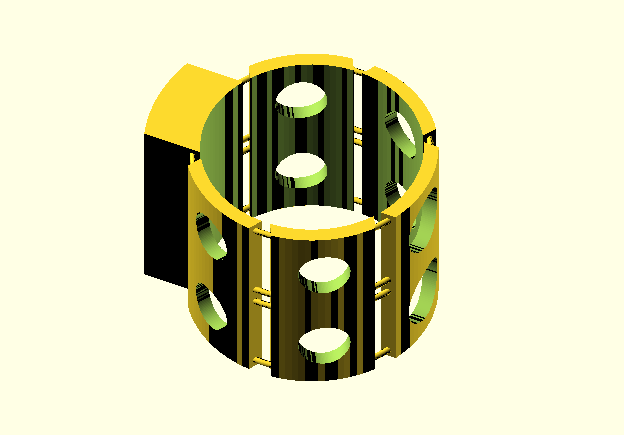
\includegraphics[width=0.4\textwidth]{graphics/bracelet-01.png}
    \end{center}
    \caption{Bracelet design [PRELIM].\label{fig:fig1}}
\end{figure}

It is use cases no. 3 and 4 that we consider for their potential musicality and the applicability of musical-inspired pattern design. These patterns must be suitable for low resolution vibrotactile arrays (in our case a circular array comprising 6 x 2 vibe motors that encircle the wrist.\\

Mapping of types of things that are commonly expressed using SMN, entities such as notes with durations, parts, and instruments need to translated, or mapped, from the music domain to that of vibrotactile devices. This mapping has proven to be useful and appears to lead to interesting possibilities for pattern design for these devices.   


%%%%%%%%%%%%%%%%%%%%%%%%%%%%%%%%%%%%%%%%%%%%%%%%%%%%%%%%%%%%%%%%%%%%%%%%%%%%%%
\section{Related Work}

\subsection{Haptic feedback and communication}
Haptic communication through force feedback is a common technique used in gaming. It purpose is to introduce the sense of touch to interactions such as movement through space, collision with, and proximity to, objects, and notification of awarding of game points and of proximity to dangerous situations. Touch can add sensual aspects and realism to computer interactions and may be useful in reducing sensory overloads from other perceptual modalities such those used in graphical interfaces \cite{oakley2000putting}, or with devices too small to have large visual displays.\\

Oakley provides a useful taxonomy of haptic-related terms, such as proprioceptive, kinesthetic and tactile. Haptic is a general term relating to the sense of touch, while tactile is more specific and relates to the sensation of pressure rather than that of temperature or pain \cite{oakley2000putting}. The largest organ of the human body is the skin and has great potential for the transmittal of information and sensation \cite{lindeman2006wearable} \cite{brewster2004tactons}.\\

Haptic feedback has a long history in the design of computer mice and of other hand controllers \cite{yang2005novel}. Touch is of course useful in generating intimacy in normal social situations \cite{bronner1982haptic}. It can also be used to coordinate action in online or gaming situations \cite{ho1998experiment}. The new Apple Watch also enables wearers to communicate their heartbeat to others wirelessly \cite{marks2014pulse}.\\

\subsection{Wearable vibrotactile devices}
Typically, haptic devices beyond experimental contexts are either wearable or holdable. One challenge of wearable devices is how to encourage people to wear them. People tend to be very particular about the look and feel of devices that provide potentially intimate notifications.\\ 

The purposes of such devices are varied and include emulation of attention-getting practices such as the squeezing of wrists, touching of shoulders and pats on arms. As Baumann notes, such social gestures may include a wealth of sub-texts including urgency, affection and reinforcement of social hierarchies \cite{baumann2010emulating}.\\

Due to their potentially non-disruptive nature, vibrotactile devices could aid in tasks in which the user's attention might be devoted to some other task, such as navigation, or gameplay, or in situations where visual information is scarce or non-existent, as with the blind \cite{ertan1998wearable}.  Devices vary in the degree of body contact they provide. The ability of he body to perceiver vibrotactile stimuli varies greatly between regions of the body dues to variation in skin receptor density \cite{lindeman2006wearable}. Work has been also done in wide-area stimulation instead of areas of the body where receptor density is greatest, such as the tips of the fingers and lips.\cite{lindeman2004towards}. Vibrational patterns suitable for a wrist device are much less complex than those designed for auditory perception due to the constrained perceptual channel of the cutaneous and kinaesthetic possibilities of the wrist compared to that of our ears.\\  

\subsection{Tactile authoring for vibrotactile devices}
Wearable tactile devices are increasing in popularity, especially for handsfree applications. Tools for authoring of tactile patterns for these devices makes the job much easier. Paneels, et al. describe a system for easy prototyping of tactile patterns based on a graphic representation of the shape of the device. A vibrotactile editor represents vibration pitch by vertical placement of notes, as in SMN. They describe the difficulty in designing such patterns by non-experts since it pre-supposes knowledge of music notation as well as other technical area like waveform design. Nor does the system support tactile design for multiple actuators \cite{paneels2013tactiped}.\\

Brown examines how musical techniques can be applied to tact on design. Tactons are structured vibrotactile messages designed to communicate information non-visually. They are the tactile counterpart of visa icons \cite{brewster2004tactons}. She examines the role of tactile dynamics and concludes that they should be combined with consideration of other vibrotactile parameters such as duration, roughness and rhythm \cite{brown2006tactile}.\\ 

Gunther explores the notion of tactile composition, which he views as a novel coupling of haptics technology and music, for the purpose of creating aesthetically appealing tactile compositions. He notes the close relation between sound and touch in all musical performance. He later describes the complex psychophysics that informs the composition of spatio-temporal patterns on the skin  \cite{gunther2003cutaneous}. 

\subsection{Authoring for multiple actuator devices}
Devices that contain several vibrotactile actuators are common \cite{gunther2003cutaneous}, \cite{lindeman2004towards}, \cite{lindeman2006wearable}, \cite{ertan1998wearable}, \cite{brown2007tactons}, These tend to be placed at various locations around the body, or in tiny pin arrays suitable for fingertip stimulation \cite{brewster2004tactons}. The design of tactile patterns depends on the configuration and placement of the actuators. A wrist-worn bracelet similar to our device is described in \cite{paneels2013tactiped}. The purpose of having multiple actuators is distribute notifications of events in places around the body that will be noticed while people do other physically or cognitively demanding activities \cite{lindeman2006wearable}, to transmit symbolic information similar to the fingertip sensing of braille \cite{brewster2004tactons}, to develop skills with polyphonic rhythms  \cite{holland2010feeling}, providing feedback for digital musical instruments \cite{marshall2006vibrotactile} \cite{schumacher2013vibrotactile}, or to create aesthetically appealing patterns for the skin \cite{gunther2003cutaneous}.


%%%%%%%%%%%%%%%%%%%%%%%%%%%%%%%%%%%%%%%%%%%%%%%%%%%%%%%%%%%%%%%%%%%%%%%%%%%%%%
\section{Designing patterns using standard music notation}

\subsection{Introduction}
In this research pattern design starts with SMN with the text-based music engraving and compositional tool Lilypond \cite{nienhuys2003lilypond}, which is a similar process to writing papers using the document preparation system LaTex. The output of Lilypond follows musical conventions and is high quality. Like LaTex, its textual input can be easily version-controlled. Once learned to a rudimentary level Lilypond is a useful tool for experimenting with SMN.  The application Frescobaldi [http://frescobaldi.org] was used as a sheet music text editor to Lilypond. Lilypond can easily output MIDI code. This MIDI code can be used to drive the actuator array in the vibrotactile bracelet using the standard Arduino MIDI library. The complete workflow for is to first compose music in Frescobaldi/Lilypond, then output a MIDI file from the Lilypond source, import this MIDI file into a track in Ableton Live, send a MIDI stream out from Ableton into a dedicated USB MIDI cable and then read this MIDI data in Arduino, using MIDI-read() function. The workflow proved to be quite workable as an experimental technique.

\subsection{Basic mapping conventions}
Our notational approach for our wrist-wearable device is to follow standard music notation (SMN) conventions and to see where these conventions lead us:

\begin{itemize}
\item Represent time horizontally form left to right. Notes to the right occur later.
\item A note represents an activation of a component. A component can be of several types (vibe motor, LED, etc.). Place notes on normal, five line staves.
\item Represent note durations by note type (for example, quarter, half and whole notes), dots and by ties between notes of the same pitch.
\item If notes are pitched, indicate their pitch through their vertical placement on a staff. If notes are unpitched, represent different components (e.g. different types of vibe motors or LEDs) using various note heads or annotations.
\item Different \textit{parts} are on separate staves. One tactor type playing the same notes at the same time represents playing in \textit{unison}. For example, eight tactors playing in unison can be represented as one part; there is no need to repeat the same information eight times. 
\item Simultaneous notes, or \textit{chords} are stacked vertically, as in SMN.
\end{itemize}

As a second step we need to translate the nomenclature from our domain of vibrating wrist wearables to that of standard music. The flowing table indicates the mapping we have applied from our domain to that of music notation:

\begin{table}[htbp]
\caption{Vibrotactile vs Music notation terms}
\small
\centering
\begin{tabular}{@{}ll@{}}
\toprule
Vibrotactile term & SMN term \\ 
\midrule
Activation of one component & Note \\
Activation duration & Note duration \\
One type of component & Instrument \\
Series of activations for one instrument & Part \\
Frequency of an activation & Pitch \\
Simultaneous activations w/ multiple pitches & Chord \\ 
\bottomrule
\end{tabular}
\end{table}

Therefore, the basic components of music are present even with a wrist-wearable vibrotactile device that does not, at first, seem to have a musical aspect: \textit{notes} with durations, pitched notes played on various discrete \textit{instruments} (vibe motors and LED lights), various \textit{parts,} or \textit{voices,} played in polyphonic \textit{compositions} and the dynamics of various parts playing together. Pitch differentials are also possible with tactors, as their frequency can be modelled using standard pulse-width modulation (PWM) techniques. \cite{lindeman2006wearable}\\

\subsection{Pitch}
Vertical placement for normal, pitched notes in SMN indicates their pitch. The pitch of a note is one of its primary psychoacoustic attributes, along with its duration, loudness and timbre. Unpitched notes are those for which the frequency is indeterminate, too complex or unrelated to the pitch contours of melodic or harmonic parts. The perception of pitch in vibrotactile devices differs from that of normal acoustic instruments. The number of frequency differences is much reduced and depends on amplitude. There may be as few as five frequency distinctions possible with cutaneous perception, or as many as ten \cite{van2003distilling}. The skin's maximal frequency response occurs around 250 Hz \cite{gunther2003cutaneous}. So it is clear that the chromatic range of pitches and frequencies over many octaves as normally represented using music notation is not suitable for cutaneous perception, but that some variation in pitch is possible. 

\subsection{Intensity}
As with aural music, suitable intensities for vibrotactile devices range from those that are barely perceptual to those that become uncomfortable. Considerations of the amplitude envelope (amplitude, delay, sustain, release, or ADSR) and with amplitude modulations such as tremolo or pitch modulations like vibrato \cite{gunther2003cutaneous}. 

\subsection{Duration}
If vibrotactile notes are of short duration they are perceived as sharp taps or jobs in the skin \cite{gunther2003cutaneous}. MORE to be added HERE.

\subsection{Vibrotactile clues}
As noted above one of the primary use cases for our vibrotractile device is offer vibrotactile clues about where crystals and treasures can be found within transmedia-inspired gameplay. These clues are intended to provide the following messages to the game-player: 'Go this way / don't go that way,'
'You're getting warmer / you're getting colder,' and 
'You're performing the correct movement / you're performing the wrong movement.'\\

The first two of these are spatial in nature and are also metaphorical, in that they refer to navigating through some kind of virtual space. The last one is kinesthetic in that it refers to moving your limbs through space in some preferred way. Music does not lend itself, on first examination, to these sorts of concepts or metaphors. It is unclear at first what music that could be interpreted as 'go this way' might look like. It seem though that it should incorporate some notion of movement through a space. SMN tends not to focus too much on such spatial considerations. Basic, notated music has no spatial dimensions. There is no specification of where instruments or performers are arranged in space. Instruments are usually placed together in cluster (as opposed to being evenly dispersed amongst performers playing other parts) but this is a performance convention and is outside of the notation itself.\\

\subsection{Music with one spatial dimension (1D = linear)}
Music with one dimension is that which instruments follow some kind of spatial linear progression, such as pan or a sweep. 

Figure ~\ref{fig:arrowsMoving00}. shows one vibe motor activating in a simple rhythm with a simple, rhythmic pitch change. By the conventions of music notation it is clear that there is a regular repetitive rhythm represented. Of course, to know even this requires at least a rudimentary knowledge of music notation. 

%\begin{figure}[htb]
%    \begin{center}
%        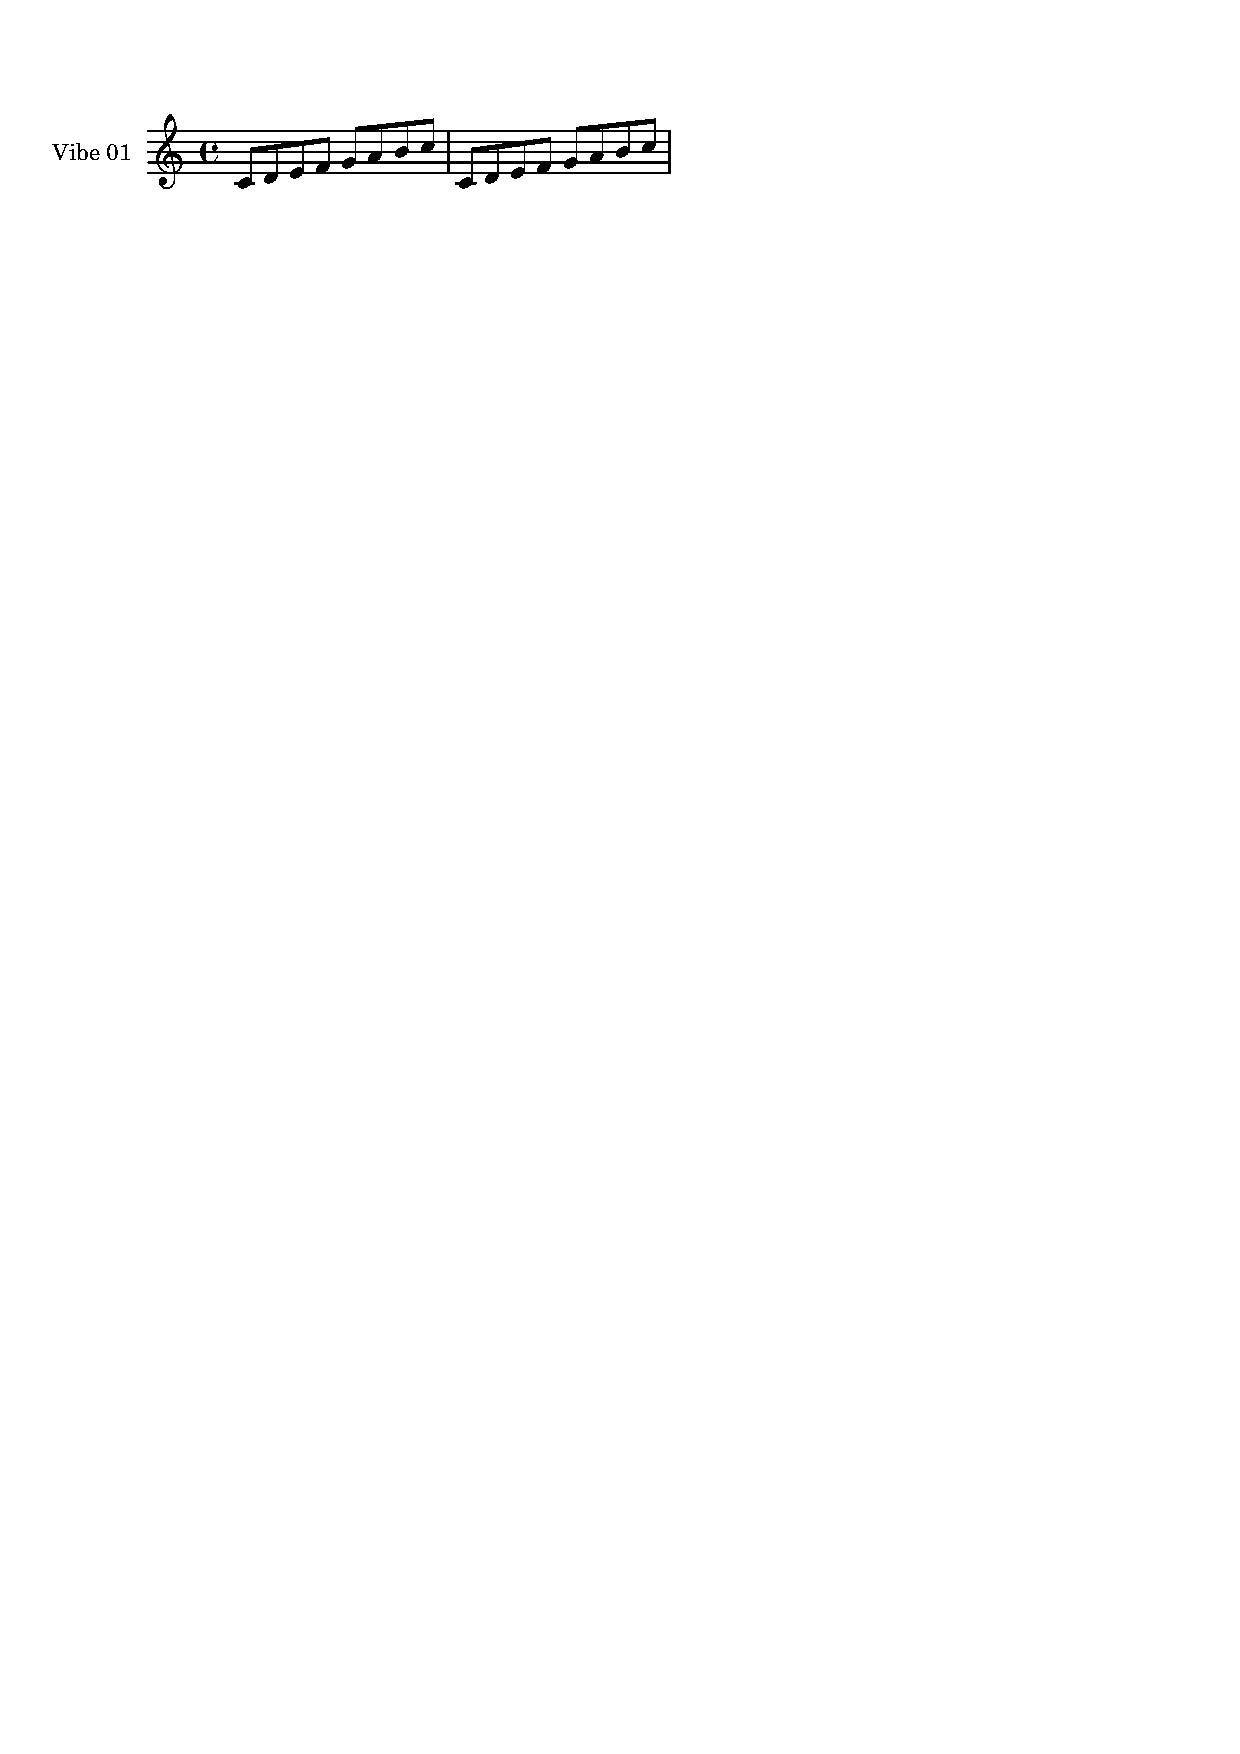
\includegraphics[width=0.4\textwidth]{graphics/scaleArduino-01.pdf}
%    \end{center}
%    \caption{Simple scale for a pitched Arduino component.\label{fig:fig2}}
%\end{figure}

%\begin{figure}[htb]
%    \begin{center}
%        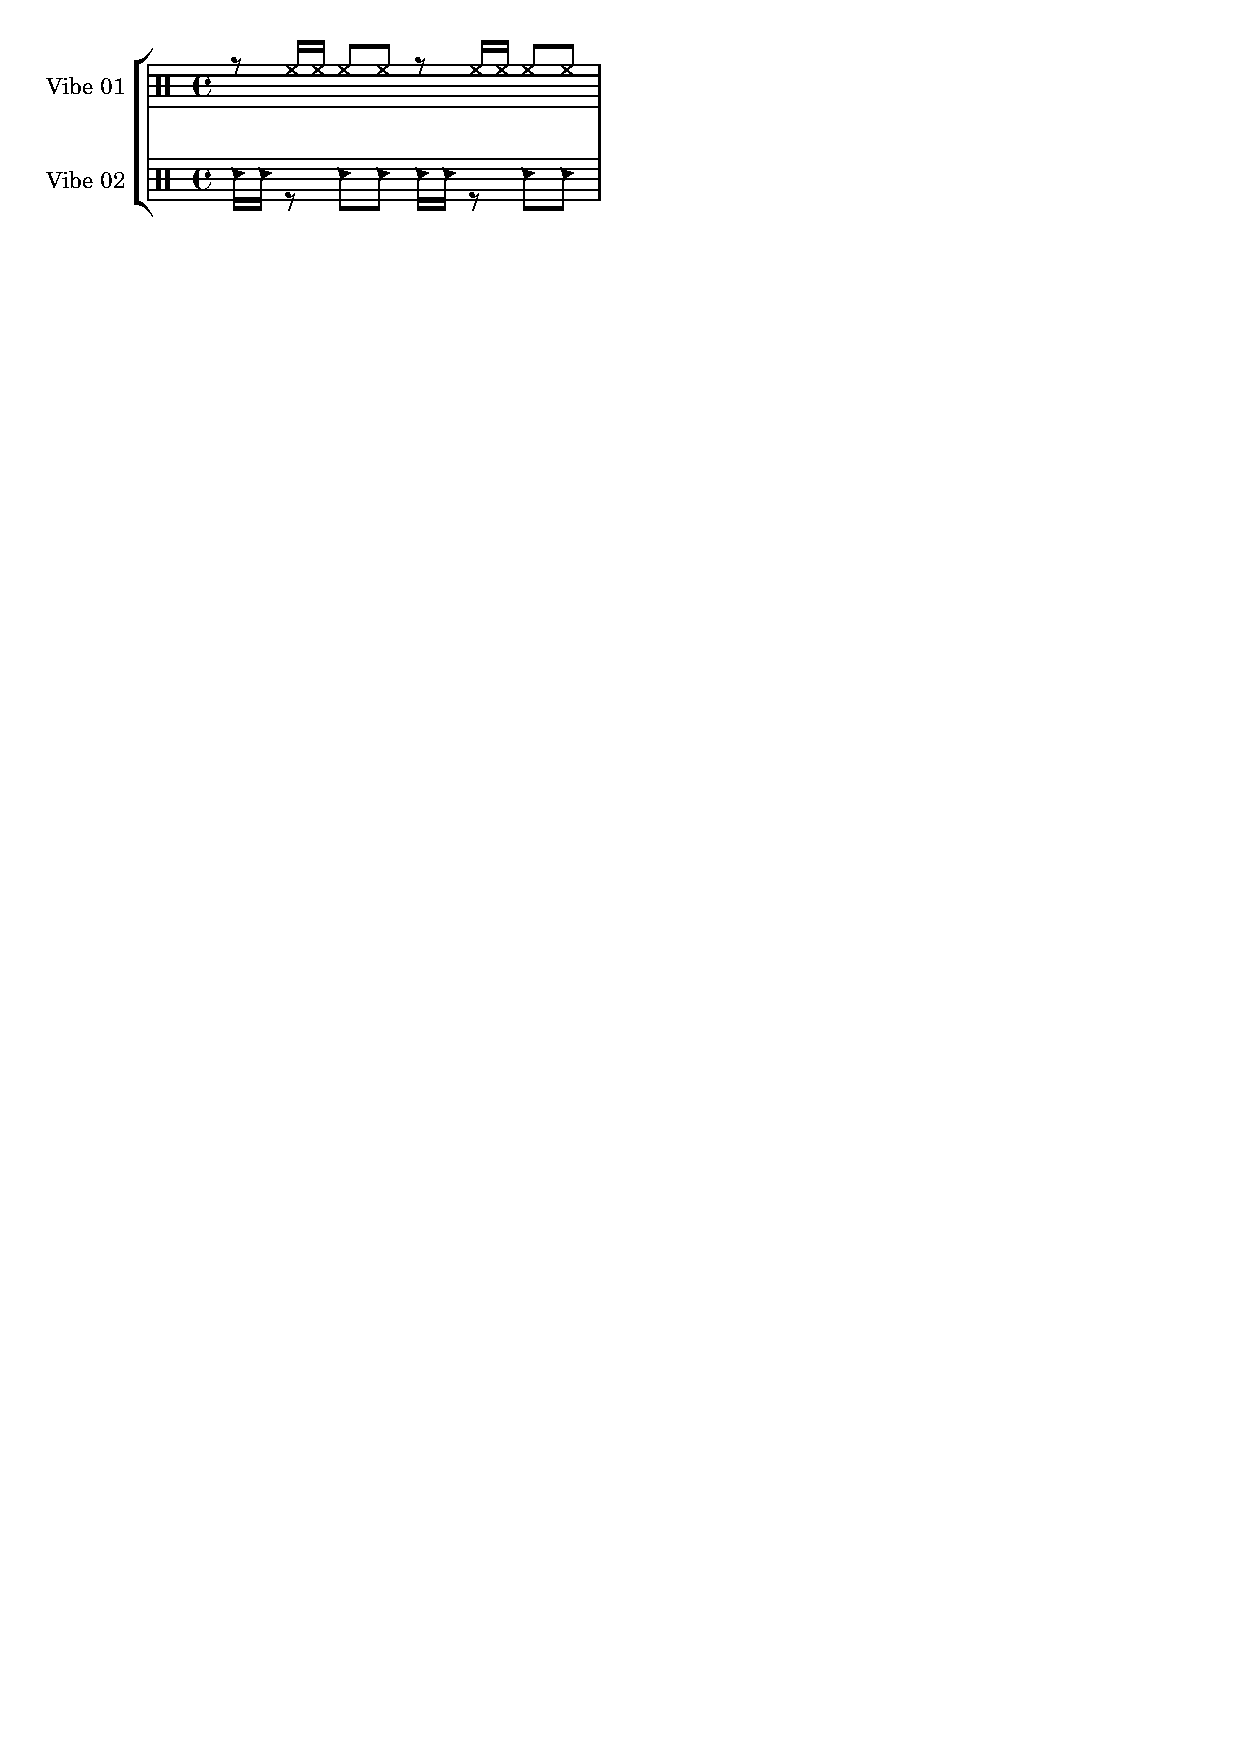
\includegraphics[width=0.4\textwidth]{graphics/drums1-simple.pdf}
%    \end{center}
%    \caption{Simple rhythm for two unpitched Arduino components.\label{fig:fig3}}
%\end{figure}

%\begin{figure}[htb]
%    \begin{center}
%        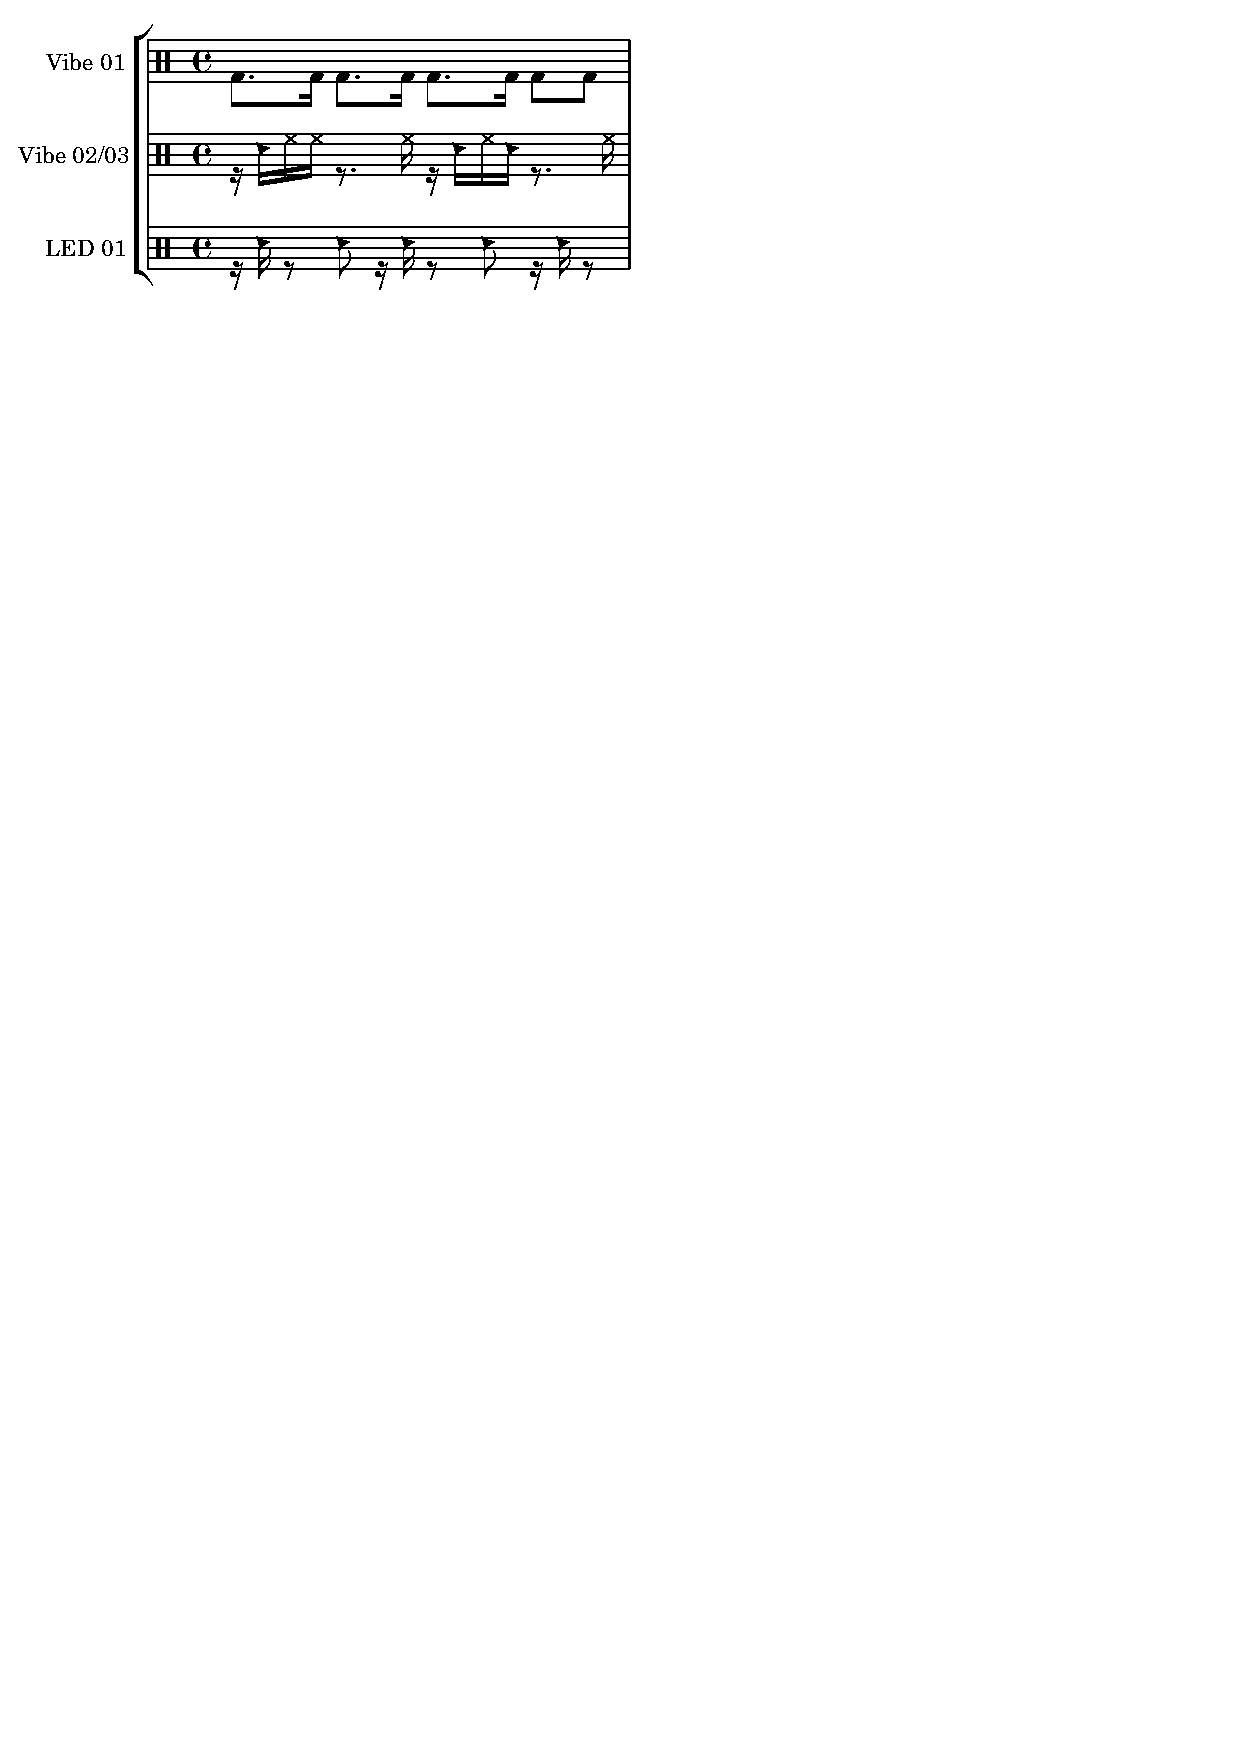
\includegraphics[width=0.4\textwidth]{graphics/drums1-multistaff.pdf}
%    \end{center}
%    \caption{Complex rhythm for three Arduino components.\label{fig:fig4}}
%\end{figure}

\begin{figure}[htb]
    \begin{center}
        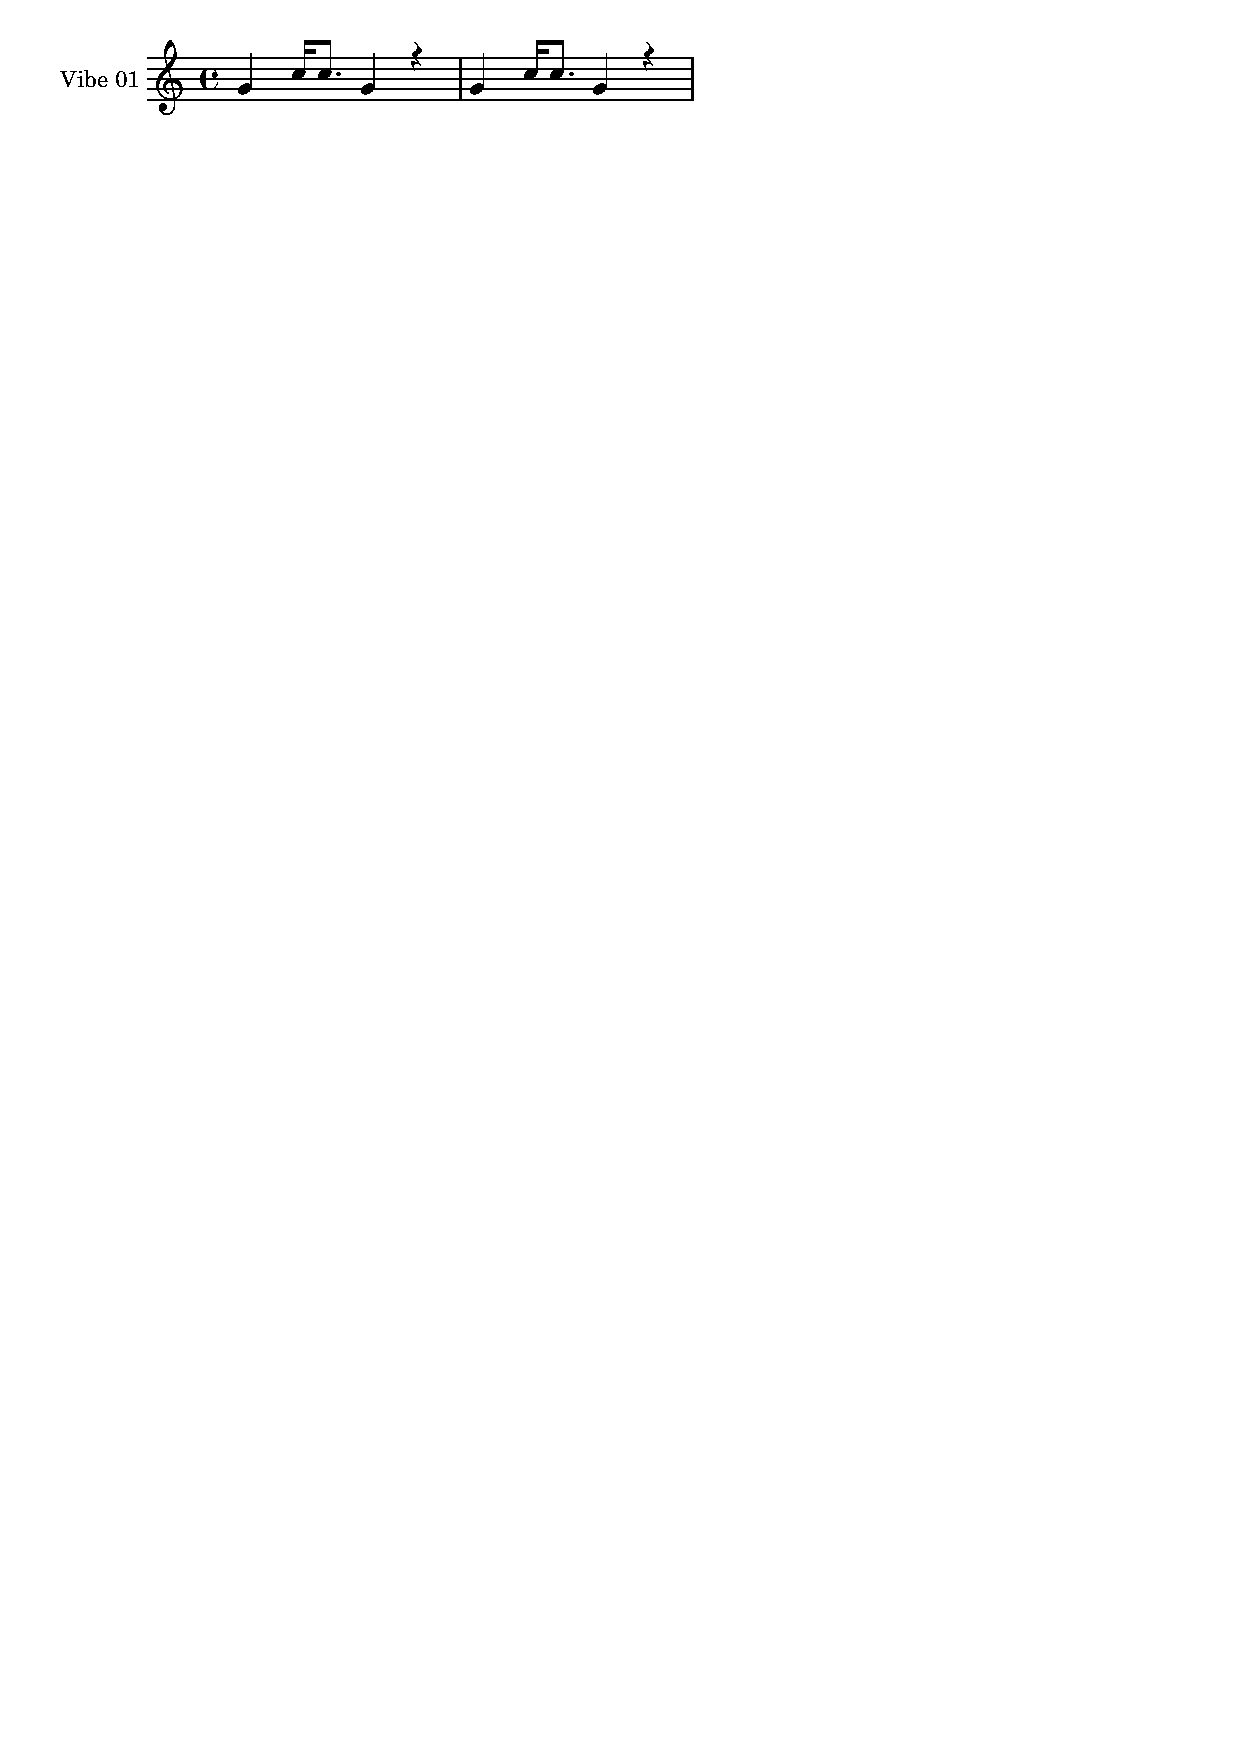
\includegraphics[width=0.4\textwidth]{graphics/arrowsMoving-00.pdf}
    \end{center}
    \caption{One vibe motor playing a simple rhythm.\label{fig:arrowsMoving00}}
\end{figure}

Figure ~\ref{fig:arrowsMoving01}. shows three vibe motors activating in a sequential motion. Note that all three are playing the same pitch. If the three separate \textit{parts} where placed on the same staff there would be confusion about which note applies to which motor. If the three motors were placed next to each other then their pulsation would have a directionality due to the physical placement of the motors. However, this directionality is less apparent in the notation itself. 
\\

\begin{figure}[htb]
    \begin{center}
        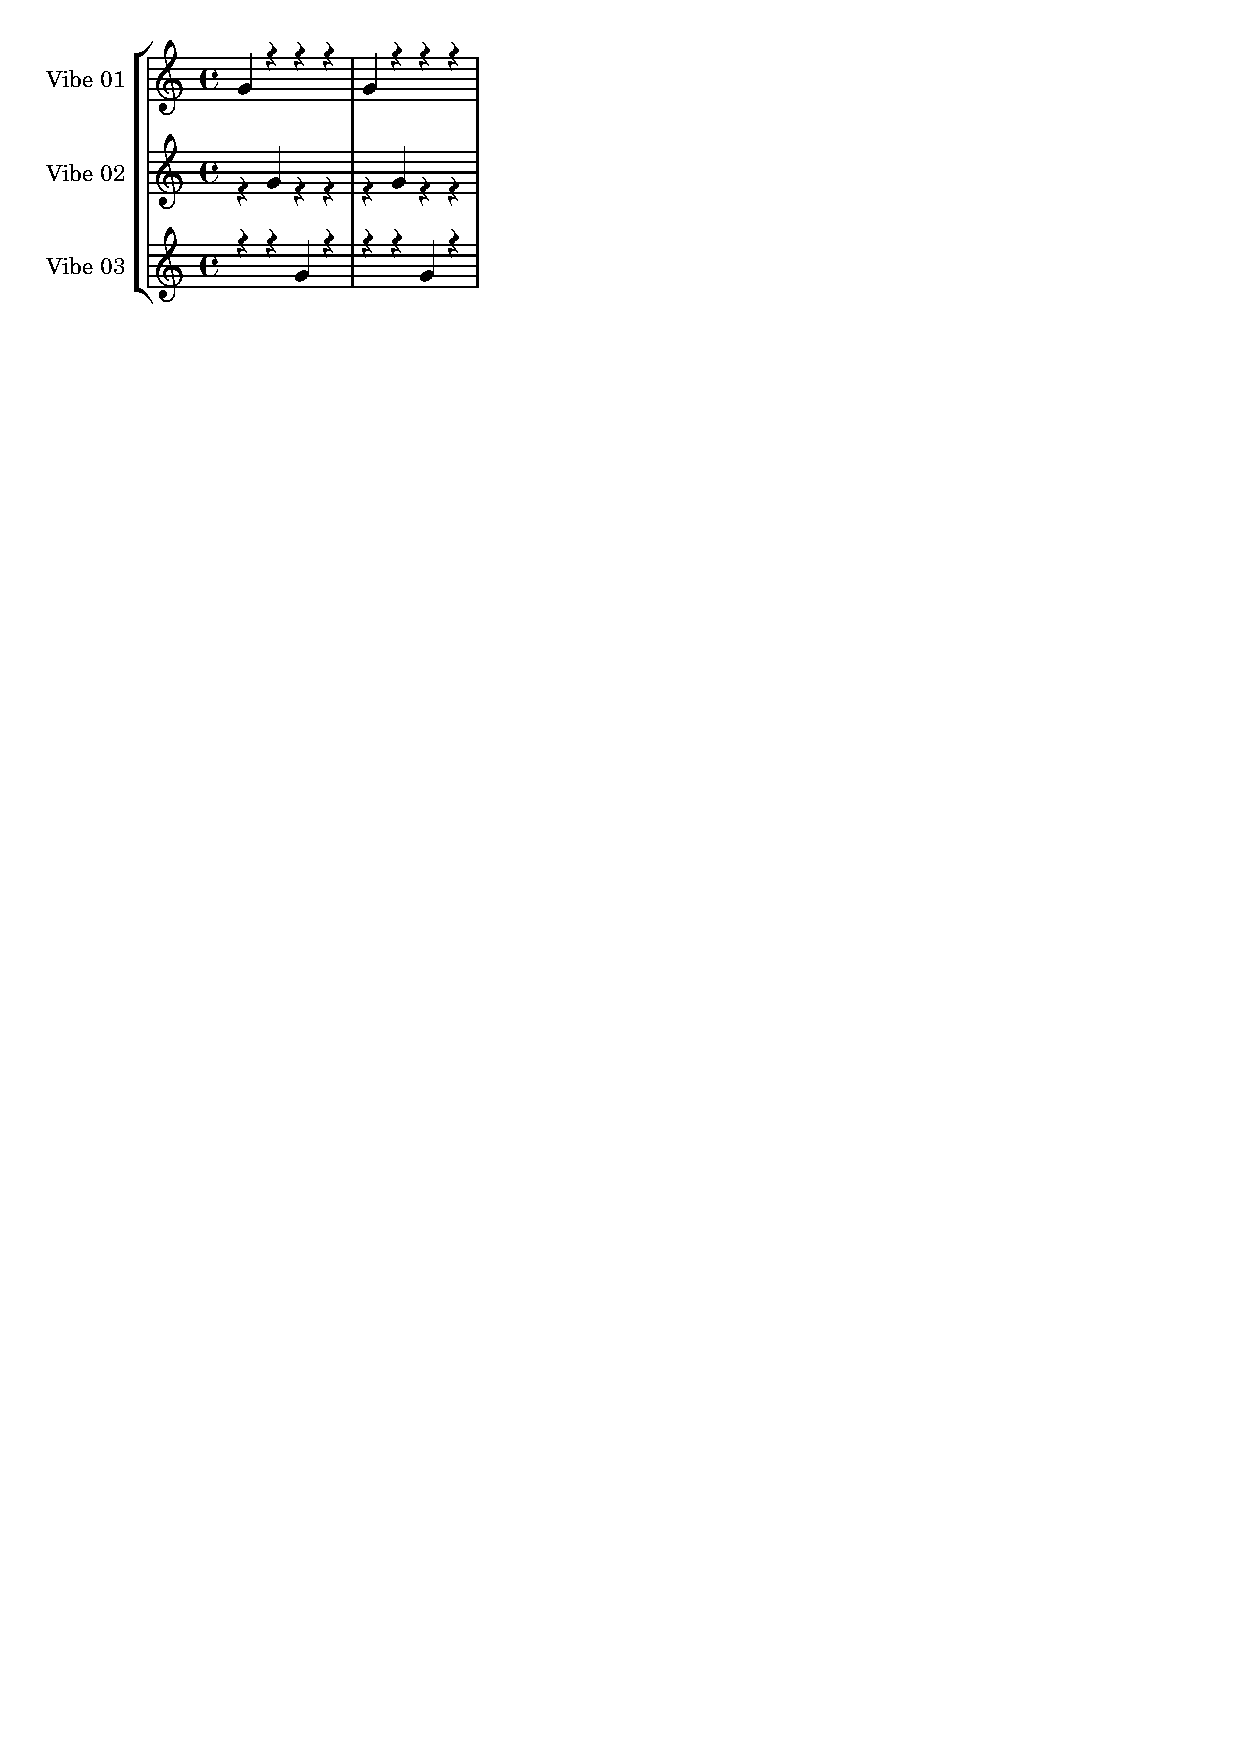
\includegraphics[width=0.4\textwidth]{graphics/arrowsMoving-01.pdf}
    \end{center}
    \caption{Threes vibes activating sequentially.\label{fig:arrowsMoving01}}
\end{figure}

The only indication that Vibe 02 might be placed after Vibe 01 is because of the numbering system. Note that the spatial dimension described is only one dimensional. The vibe motors are arranged along a line. With vibe bracelets what is desirable is to represent two dimensions such that patterns can be created across the skin. It would be useful if the spatial dimension Is there any dimension is standard musical notation that indicates 2D spatial placement of instruments? 

\subsection{Music with two spatial dimensions (2D = planar)}

This highlights a problem with using musical notation for describing the activation of spatially separate vibe motors: when you want to describe the movement of vibrations spatially then where the vibe motors are located in space is essential to represent using the notation. With pitched notation the pitch, timing and rhythm of the music tends to be its most important aspect. The spatial placement of the instruments playing different parts is less of a concern. How then can vibe motors activating in a spatially differentiated manner be represented -- compactly and efficiently -- using standard music notation?\\

MORE to be added HERE...

%%%%%%%%%%%%%%%%%%%%%%%%%%%%%%%%%%%%%%%%%%%%%%%%%%%%%%%%%%%%%%%%%%%%%%%%%%%%%%
\section{Discussion}



%%%%%%%%%%%%%%%%%%%%%%%%%%%%%%%%%%%%%%%%%%%%%%%%%%%%%%%%%%%%%%%%%%%%%%%%%%%%%%
\section{Future Work}


Our work consists of quick interation of devices and authoring of activation patterns for a several devices. This work is motivated by both research as well as aesthetic considerations. Pattern authoring depends crucially on the nature of the device being authored for and its purpose. We consider two aspects that seem particularly promising for future development in this area: the design of vibrotactile patterns to enhance and inform transmedia narratives, and the creation of aesthetically appealing vibrotactile patterns in a variety of musical 'genres.' Our research here only scratches the surfaces in those two areas. 


%%%%%%%%%%%%%%%%%%%%%%%%%%%%%%%%%%%%%%%%%%%%%%%%%%%%%%%%%%%%%%%%%%%%%%%%%%%%%%
\section{Conclusion}
Music notation is a finely structured notational system. It requires an expert-level of competence to read its finest level of detail, however, this type of expertise is not hard to find in cultures where notated musical composition and performance is well-established. What is much less common is cross-expertise in both music notation and vibrotactile technologies. Standard musical notation includes many dimensions but in its standard forms does not easily lend itself to inclusion of more non-musical dimensions such as required for the specification of 2 and 3D patterns for vibrotactile arrays. Howver, it appears that will some minor additions to SMN this type of authoring technique is much more appealing and culturally evocative than the alternatives. 

\section{Acknowledgements}
This work has been supported by the International Science and Technology Partnerships Canada Inc (ISTP) on the project Multi-platform Game Distribution System for Popular and Experimental Technologies (MGDS-PET) and by grants from the National Sciences and Engineering Research Council of Canada (NSERC). We would also like to thank Xenophile Media Inc., Vicki Clough, Shin-you Hou, Tegan Power, Ryan Maksymic, Takis Zourntos for the their help in the development of this project. 

%%%%%%%%%%%%%%%%%%%%%%%%%%%%%%%%%%%%%%%%%%%%%%%%%%%%%%%%%%%%%%%%%%%%%%%%%%%%%%
% REFERENCES
%%%%%%%%%%%%%%%%%%%%%%%%%%%%%%%%%%%%%%%%%%%%%%%%%%%%%%%%%%%%%%%%%%%%%%%%%%%%%%

\bibliography{CIM14_bibliography}
\bibliographystyle{CIM14}
  
\end{document}
